\section{Methoden zur Positionsbestimmung}
\label{sec:methoden}

\begin{frame}
  \frametitle{Methoden zur Positionsbestimmung}
  \begin{center}
    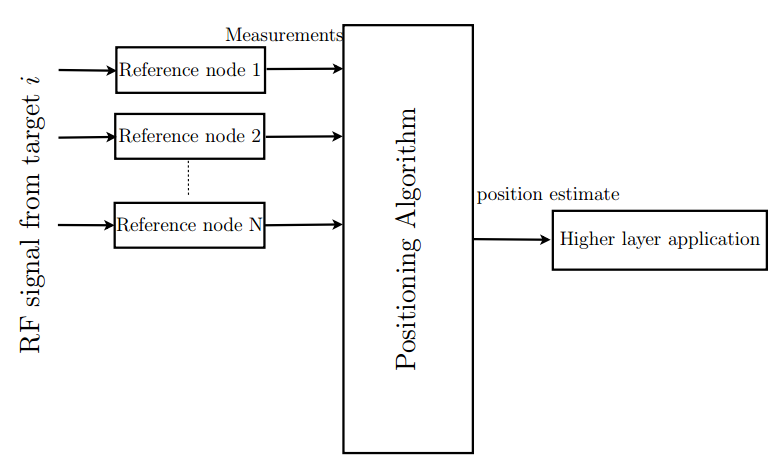
\includegraphics[scale=0.35]{img/algo_1}
  \end{center}
\end{frame}

\begin{frame}
  \frametitle{Methoden zur Positionsbestimmung}

  \begin{itemize}
  \item Anchor/Beacon Nodes
  \item Distanz
    \begin{itemize}
      \item Signalstärkemessung
      \item Hop Count
      \item Zeitmessung
    \end{itemize}
  \item Richtung
  \begin{itemize}
    \item Auftreffwinkel
  \end{itemize}
  \end{itemize}
\end{frame}

\begin{frame}
  \frametitle{Anchor/Beacon Nodes}

  \begin{itemize}
  \item Die Anchor Nodes haben eine bekannte Position (z.B. GPS oder
    fest einprogrammiert)
  \item Für ein globales 2D Koordinatensystem sind 3 nicht linear
    angeordnete Anchor Nodes erforderlich, für ein 3D KS entsprechend
    4.
  \item Es wird nun entweder ein relatives Koordinatensystem mit allen
    nicht Anchor Nodes erstellt und dann mit Hilfe dieser in ein
    globales überführt oder es wird mit Hilfe der Anchor Nodes direkt
    jede einzelne Postion der Nodes bestimmt
  \end{itemize}
\end{frame}

\begin{frame}
\frametitle{Anchor/Beacon Nodes - Vorteile/Nachteile}

\begin{itemize}
  \item Vorteile
  \begin{itemize}
    \item Für globales KS unerlässlich
    \item Vereinfachung der Positionsberechnung der anderen Nodes
  \end{itemize}
  \item Nachteile
  \begin{itemize}
    \item GPS für Anchor Nodes teuer und verbraucht viel Energie
    \item Vorprogrammieren von festen Positionen bei großen
      Sensornetzen sehr aufwendig und nur bei festen Sensornetzen
      überhaupt möglich
  \end{itemize}
\end{itemize}
\end{frame}

\begin{frame}
\frametitle{Signalstärkemessung (RSSI)\footnote{Received Signal Strength Indication}}

\begin{itemize}
  \item Nutzt die Tatsache das in einem Kabellosen SN jeder Knoten
    sowohl senden als auch empfangen kann
  \item Da die Signalstärke konstant quadratisch zur Entfernung
    abnimmt, ist theoretisch eine genaue Entfernungsmessung möglich
  \item In der Praxis verhindern jedoch Störstrahlung und die
    Dämpfung/Reflexion von Hindernissen eine genaue Messung
\end{itemize}
\end{frame}

\begin{frame}
\frametitle{Signalstärkemessung (RSSI)\footnote{Cameron Whitehouse. The design of calamari: an ad-hoc localization
system for sensor networks. Master’s thesis, University of California at
Berkeley, 2002.}}
  \begin{center}
  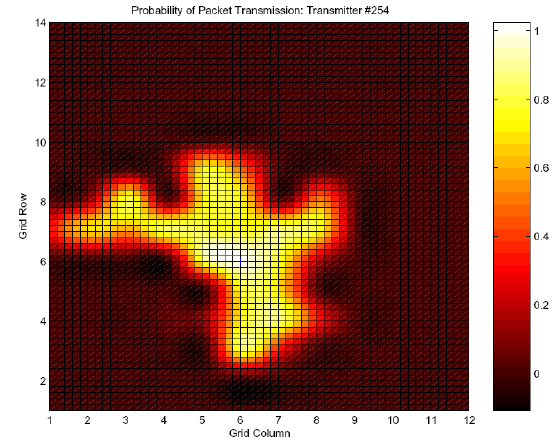
\includegraphics[scale=0.5]{img/RSSI1}
  \end{center}
\end{frame}

\begin{frame}
\frametitle{Signalstärkemessung (RSSI)}
\begin{itemize}
  \item Vorteile
  \begin{itemize}
    \item leicht zu messen
    \item keine Zusatzkosten
  \end{itemize}
  \item Nachteile
  \begin{itemize}
    \item sehr ungenau
    \item sehr störanfällig
  \end{itemize}
\end{itemize}
\end{frame}

\begin{frame}
\frametitle{Hop Count}

\begin{itemize}
  \item Basiert auf der Annahme das die Entfernung von 2 Nodes die
    miteinander kommunizieren können, kleiner ist als Reichweite der
    Sender völlig unabhängig von der gemessenen Signalstärke
  \item Es wird ein ungerichteter Graph aufgebaut mit den Nodes als
    Knoten und den direkten Verbindungen der Nodes untereinander als
    Kanten
  \item Der Hop Count $h_{i,j}$ von zwei Nodes ist der kürzeste Pfad
    zwischen diesen
\end{itemize}
\end{frame}

\begin{frame}
  \frametitle{Hop Count}

  \begin{center}
  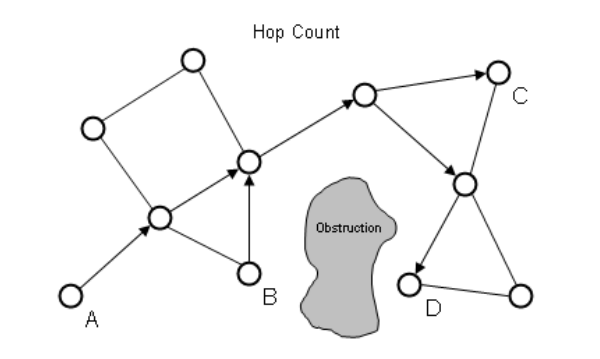
\includegraphics[scale=0.5]{img/hop_count1}
  \\~\\
  Messung A $\to$ C = 4 Hops - Messung B $\to$ D = 4 Hops
  \end{center}
\end{frame}

\begin{frame}
\frametitle{Hop Count}

\begin{itemize}
  \item Vorteile
  \begin{itemize}
    \item leicht zu messen
    \item keine Zusatzkosten
  \end{itemize}
  \item Nachteile
  \begin{itemize}
    \item selbst im Optimalfall ungenau
    \item Wenn keine direkte Sichtlinie besteht, extrem ungenau
  \end{itemize}
\end{itemize}

\end{frame}

\begin{frame}
\frametitle{Zeitmessung}

\begin{itemize}
  \item Time of Arrival (ToA)
  \item Time Difference of Arrival (TDoA)
  \item Round Trip Time of Flight (TRoF)
\end{itemize}
\end{frame}

\begin{frame}
  \frametitle{Signallaufzeitmessung (ToA)}
  \begin{itemize}
    \item Zur Messung der Entfernung wird ein Radiosignal von einem Knoten zu einem weiteren Knoten geschickt
    \item Aus der Signallaufzeit wird dann die Entfernung errechnet
  \end{itemize}
  \begin{center}
    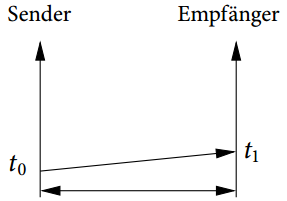
\includegraphics[scale=0.35]{img/time1}\\~\\

    $d = (t_{1} - t_{0}) \cdot c$\\~\\
    $c=299\,792\,458\;\mathrm{m/s}$
  \end{center}
\end{frame}


\begin{frame}
\frametitle{Time Difference of Arrival}
\begin{itemize}
  \item Zusätzlich zur Funkantenne sind alle Nodes hier mit Mikrofon und Lautsprecher ausgerüstet
  \item Zuerst wird ein Funksignal gesendet und der Empfänger speichert den Zeitpunkt des Empfangs $t_{radio}$
  \item Nach einer festgelegten Zeit $t_{delay}$ wird eine Tonfolge durch die Lautsprecher ausgegeben und der Empfangszeitpunkt $t_{sound}$ ebenfalls gespeichert
  \item Die Entfernung kann nun durch $d = (s_{radio} - s_{sound}) * (t_{sound} - t_{radio} - t_{delay})$ \\berechnet werden.
\end{itemize}
\end{frame}

\begin{frame}
\frametitle{Time Difference of Arrival\footnote{Janathan Bachrach and Christopher Taylor, Localization in Sensor Networks, Massachusetts Institute of Technology}}
  \begin{center}
    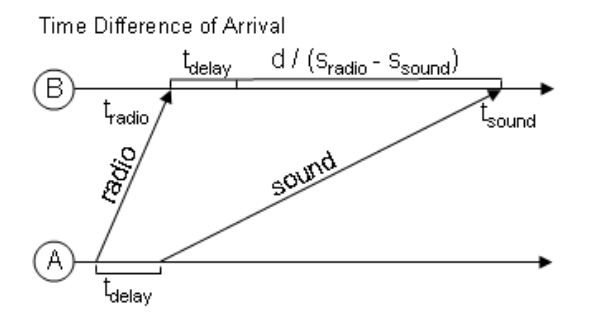
\includegraphics[scale=0.5]{img/tdoa1.png}\\~\\
  $s_{radio}=299\,792\,458\;\mathrm{m/s}$\\
  $s_{sound}=          343\;\mathrm{m/s}$
  \end{center}
\end{frame}

\begin{frame}
  \frametitle{Signallaufzeitmessung (RToF)}
  \begin{itemize}
    \item ähnlich wie bei der ToA Methode wird hier die Signallaufzeit eines Radiosignals gemessen
    \item allerdings wird im Gegensatz zur ToA das Signal auch wieder zurückgesendet einschließlich der Information über die Verzögerung
  \end{itemize}
  \begin{center}
    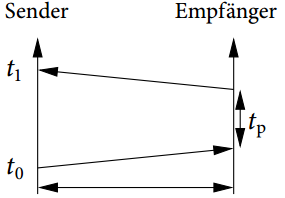
\includegraphics[scale=0.35]{img/time3}\\~\\

    $d = \frac{t_{1} - t_{0} - t_{p}}{2} \cdot c$\\~\\
    $c=299\,792\,458\;\mathrm{m/s}$
  \end{center}
\end{frame}

\begin{frame}
\frametitle{Signallaufzeitmessung}
\begin{itemize}
  \item Vorteile
  \begin{itemize}
    \item leicht zu messen 
    \item keine Zusatzkosten (ToA/RToF)
  \end{itemize}
  \item Nachteile
  \begin{itemize}
    \item zusätzliche Kosten (TDoA)
    \item zusätzliches Gewicht 
    \item zusätzlicher Raum- und Energiebedarf (TDoA)
  \end{itemize}
\end{itemize}
\end{frame}

\begin{frame}
\frametitle{Auftreffwinkel (AoA)}
\begin{itemize}
  \item Um den AoA zu messen wird am Empfangsende eine räumliche Empfangsanordnung benötigt
  \item Durch die Unterschiede der Phase bzw. der Ankunftszeiten kann dann der Winkel berechnet werden
  \item Bei ausreichender Menge und guter Anordnung der Antennen kann eine Genauigkeit von wenigen Grad Abweichung erreicht werden
\end{itemize}
\end{frame}

\begin{frame}
\frametitle{Auftreffwinkel (AoA)}
\begin{itemize}
  \item Vorteile
  \begin{itemize}
    \item Einfallswinkel für genaue Positionsbestimmung hilfreich
  \end{itemize}
  \item Nachteile
  \begin{itemize}
    \item zusätzliche Kosten
    \item zusätzliches Gewicht
    \item zusätzlicher Raum- und Energiebedarf
  \end{itemize}
\end{itemize}
\end{frame}
